%\clearpage

%\section{Background Estimation Technique}



The dominant background to the signal sample comes from \ttll\
events. Due to the presence of a second neutrino, \ttll\ events do
not have a kinematic edge at $\mt \sim \mW$. These events satisfy the
selection criteria due to real \met\ and do not depend on detector
resolution or \met\ mis-measurement effects. As a result, the
\ttll\ background is expected to be well modeled in the MC. The
prediction for this background is thus derived from MC and normalized
to the data in the \mt\ peak region. However,
there are two aspects that require dedicated corrections and are detailed
in this section:
\begin{itemize}
\item the modeling of additional jets from radiation, required to satisfy the 4-jet
selection criteria.
\item the modeling of the isolated track veto efficiency, which is
  applied to explicitly reject leptons from \W\ and $\W\To\tau$ decays
  and single prong $\tau$ decays.
\end{itemize}
The systematic uncertainty associated with the MC prediction then has two components.
One that is
derived by comparing various generators, and a second from the uncertainties on
the various correction factors used. These are described at the end of
this section.  

\subsection{Modeling of Additional Hard Jets in Top Dilepton Events}
\label{sec:jetmultiplicity}

Dilepton \ttbar\ events have 2 jets from the top decays, so additional
jets from radiation or higher order contributions are required to
enter the signal sample. The modeling of addtional jets in \ttbar\
events is checked in a \ttll\ control sample,
selected by requiring
\begin{itemize}
\item exactly 2 selected electrons or muons with \pt $>$ 20 GeV
\item \met\ $>$ 50 GeV
\item $\geq1$ b-tagged jet
\end{itemize}
Figure~\ref{fig:dileptonnjets} shows a comparison of the jet
multiplicity distribution in data and MC for this two-lepton control
sample. After requiring at least 1 b-tagged jet, most of the
events have 2 jets, as expected from the dominant process \ttll. There is also a
significant fraction of events with additional jets. 
The 3-jet sample is mainly comprised of \ttbar\ events with 1 additional
emission and similarly the $\ge4$-jet sample contains primarily
$\ttbar+\ge2$ jet events. Even though the primary \ttbar\
Madgraph sample used includes up to 3 additional partons at the Matrix
Element level, which are intended to describe additional hard jets,
Figure~\ref{fig:dileptonnjets} shows a slight mis-modeling of the
additional jets. 


\begin{figure}[hbt]
  \begin{center}
	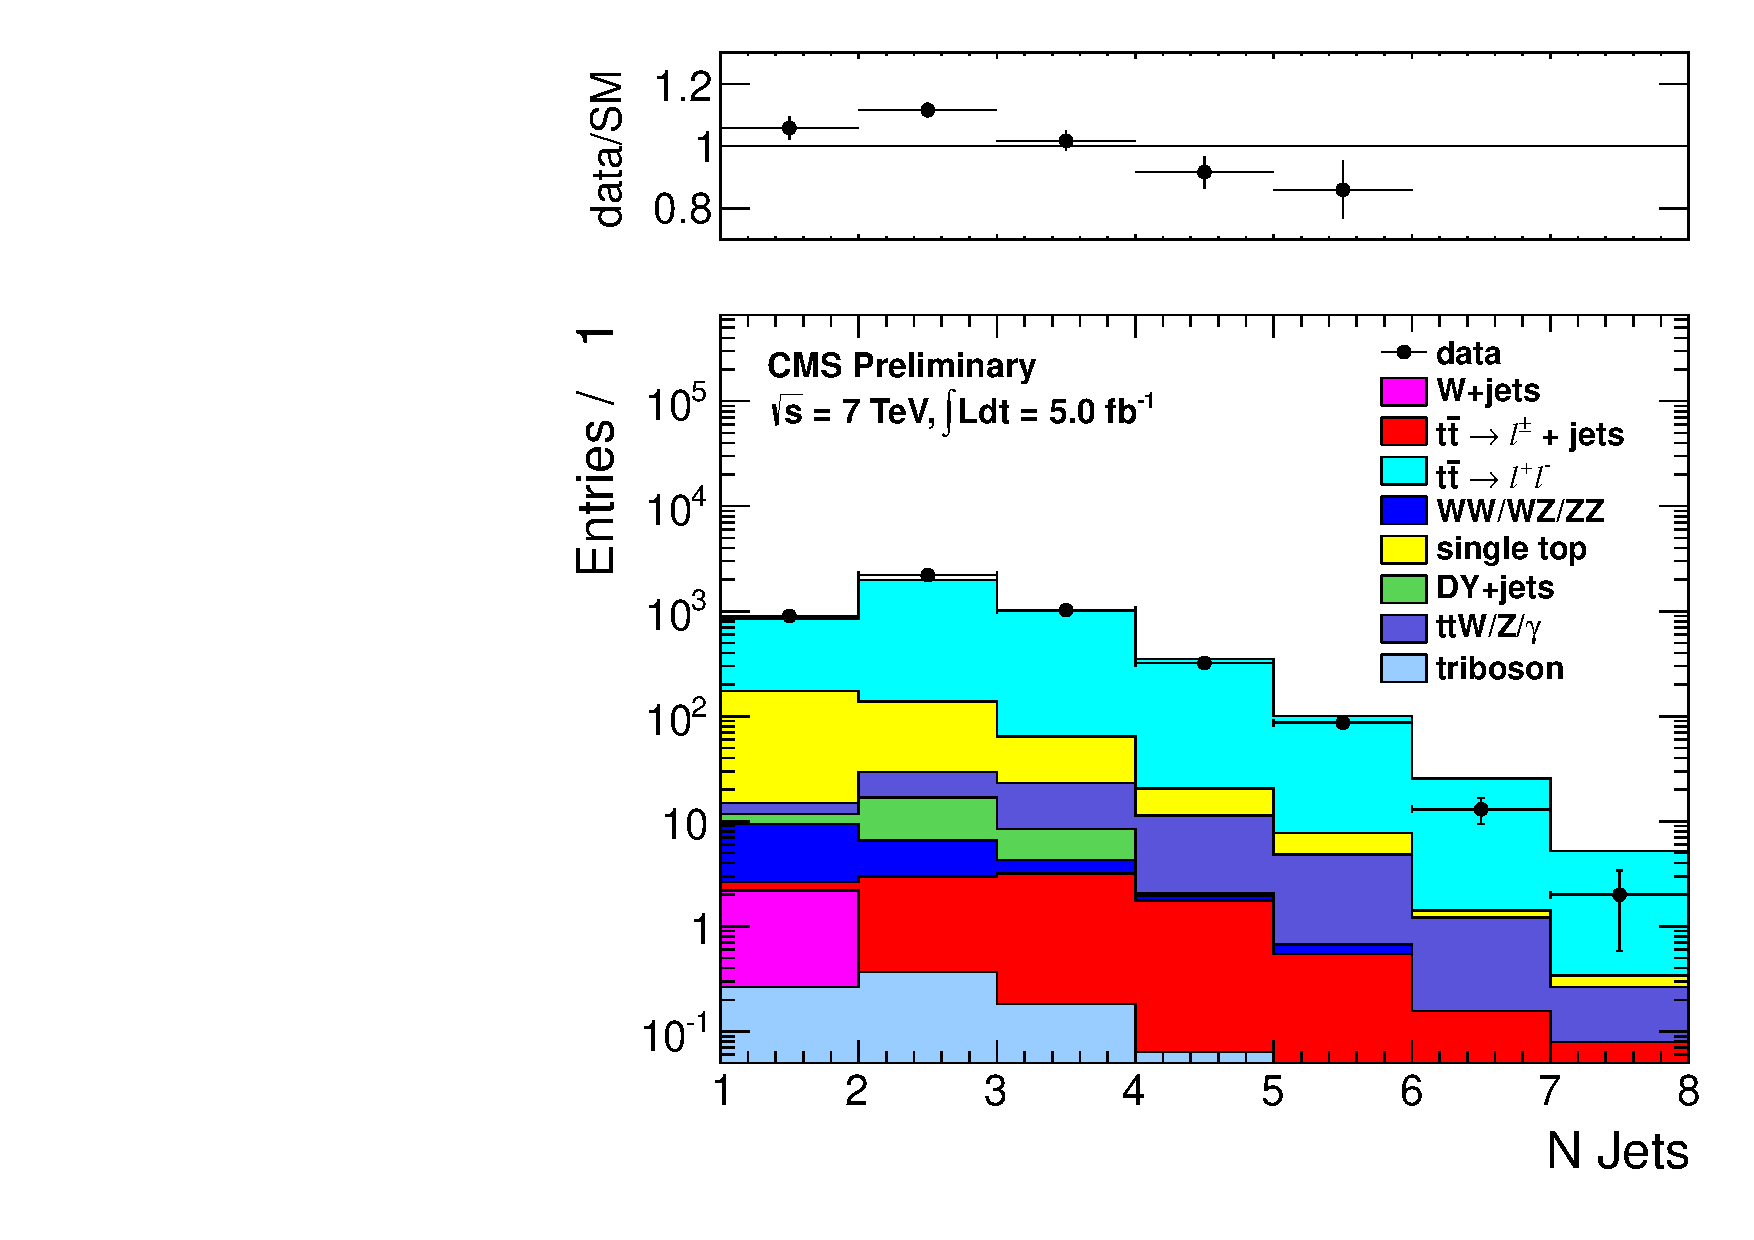
\includegraphics[width=0.5\linewidth]{plots/njets_all_dl_mueg.pdf}
	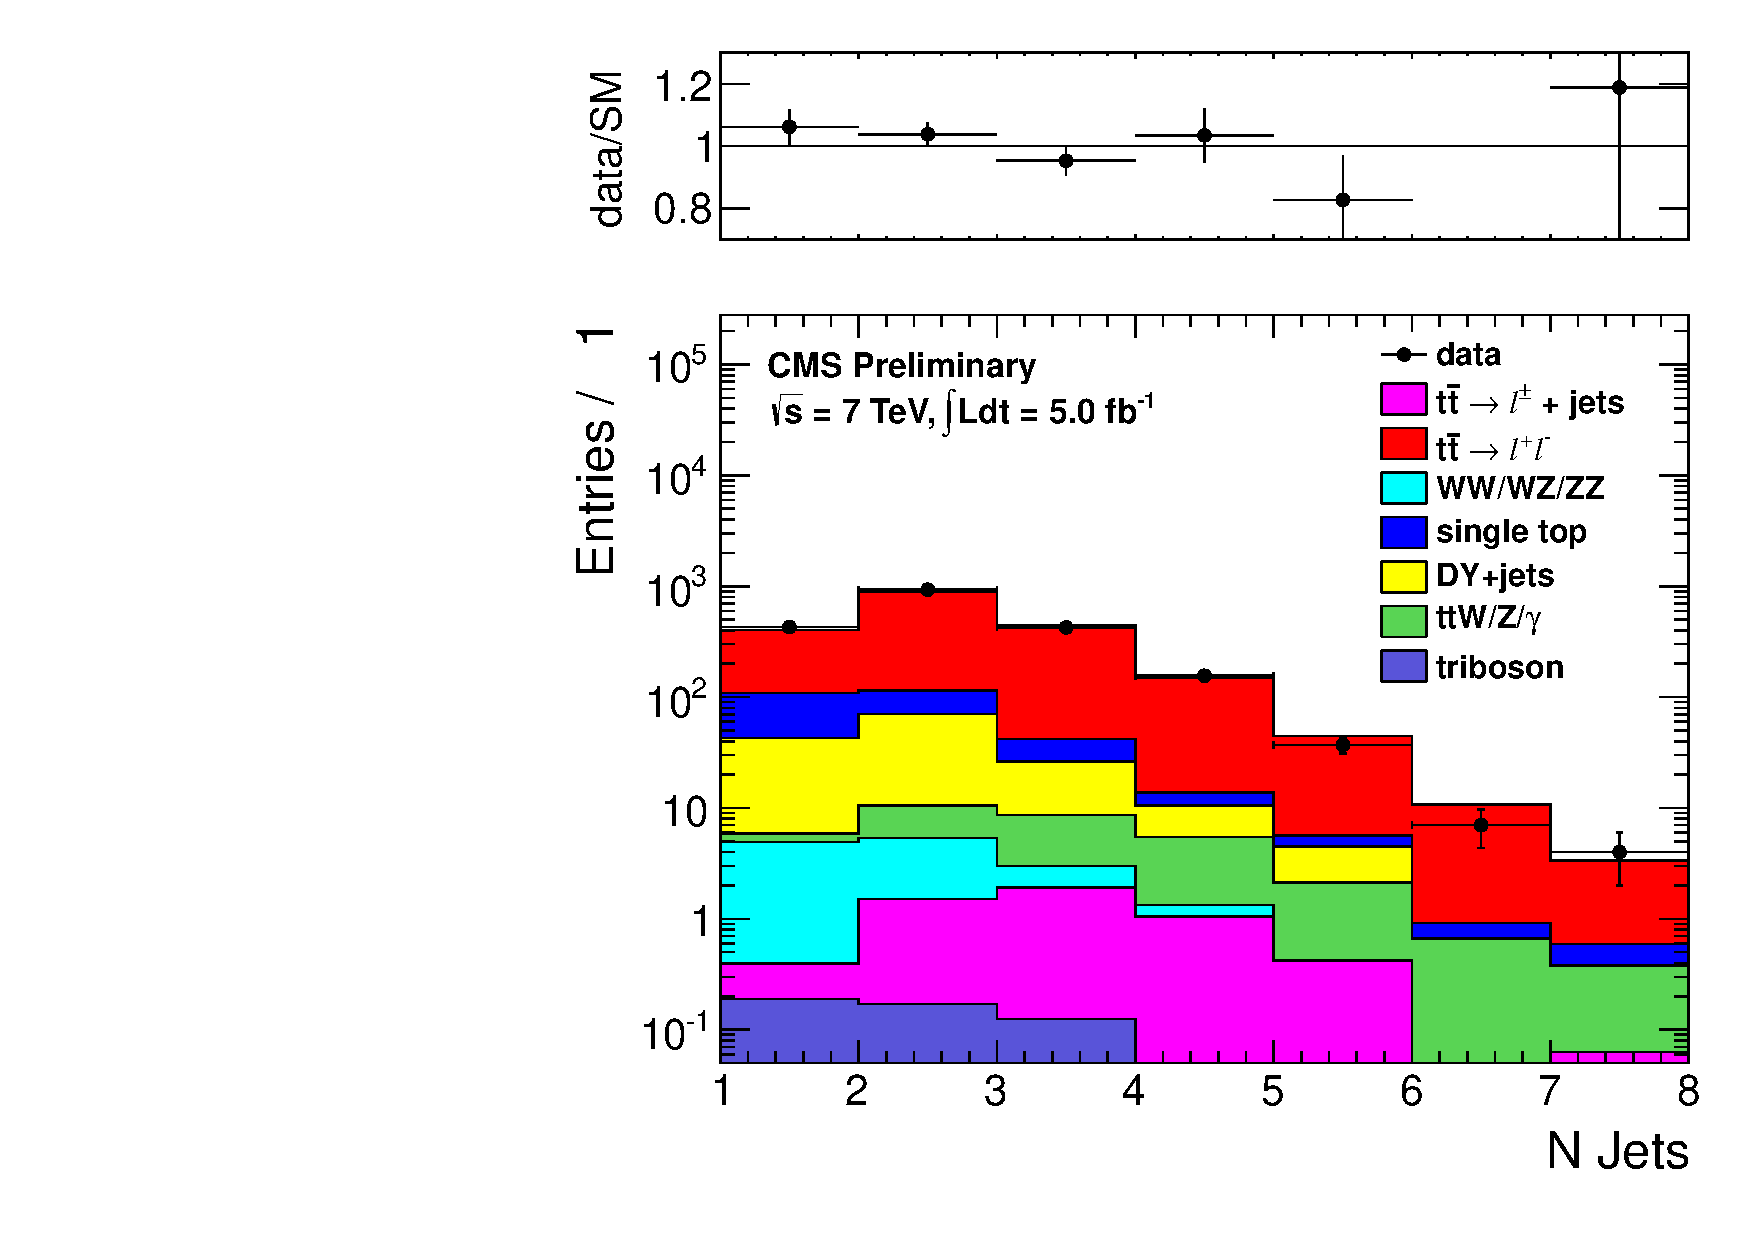
\includegraphics[width=0.5\linewidth]{plots/njets_all_dl_diel.pdf}%
        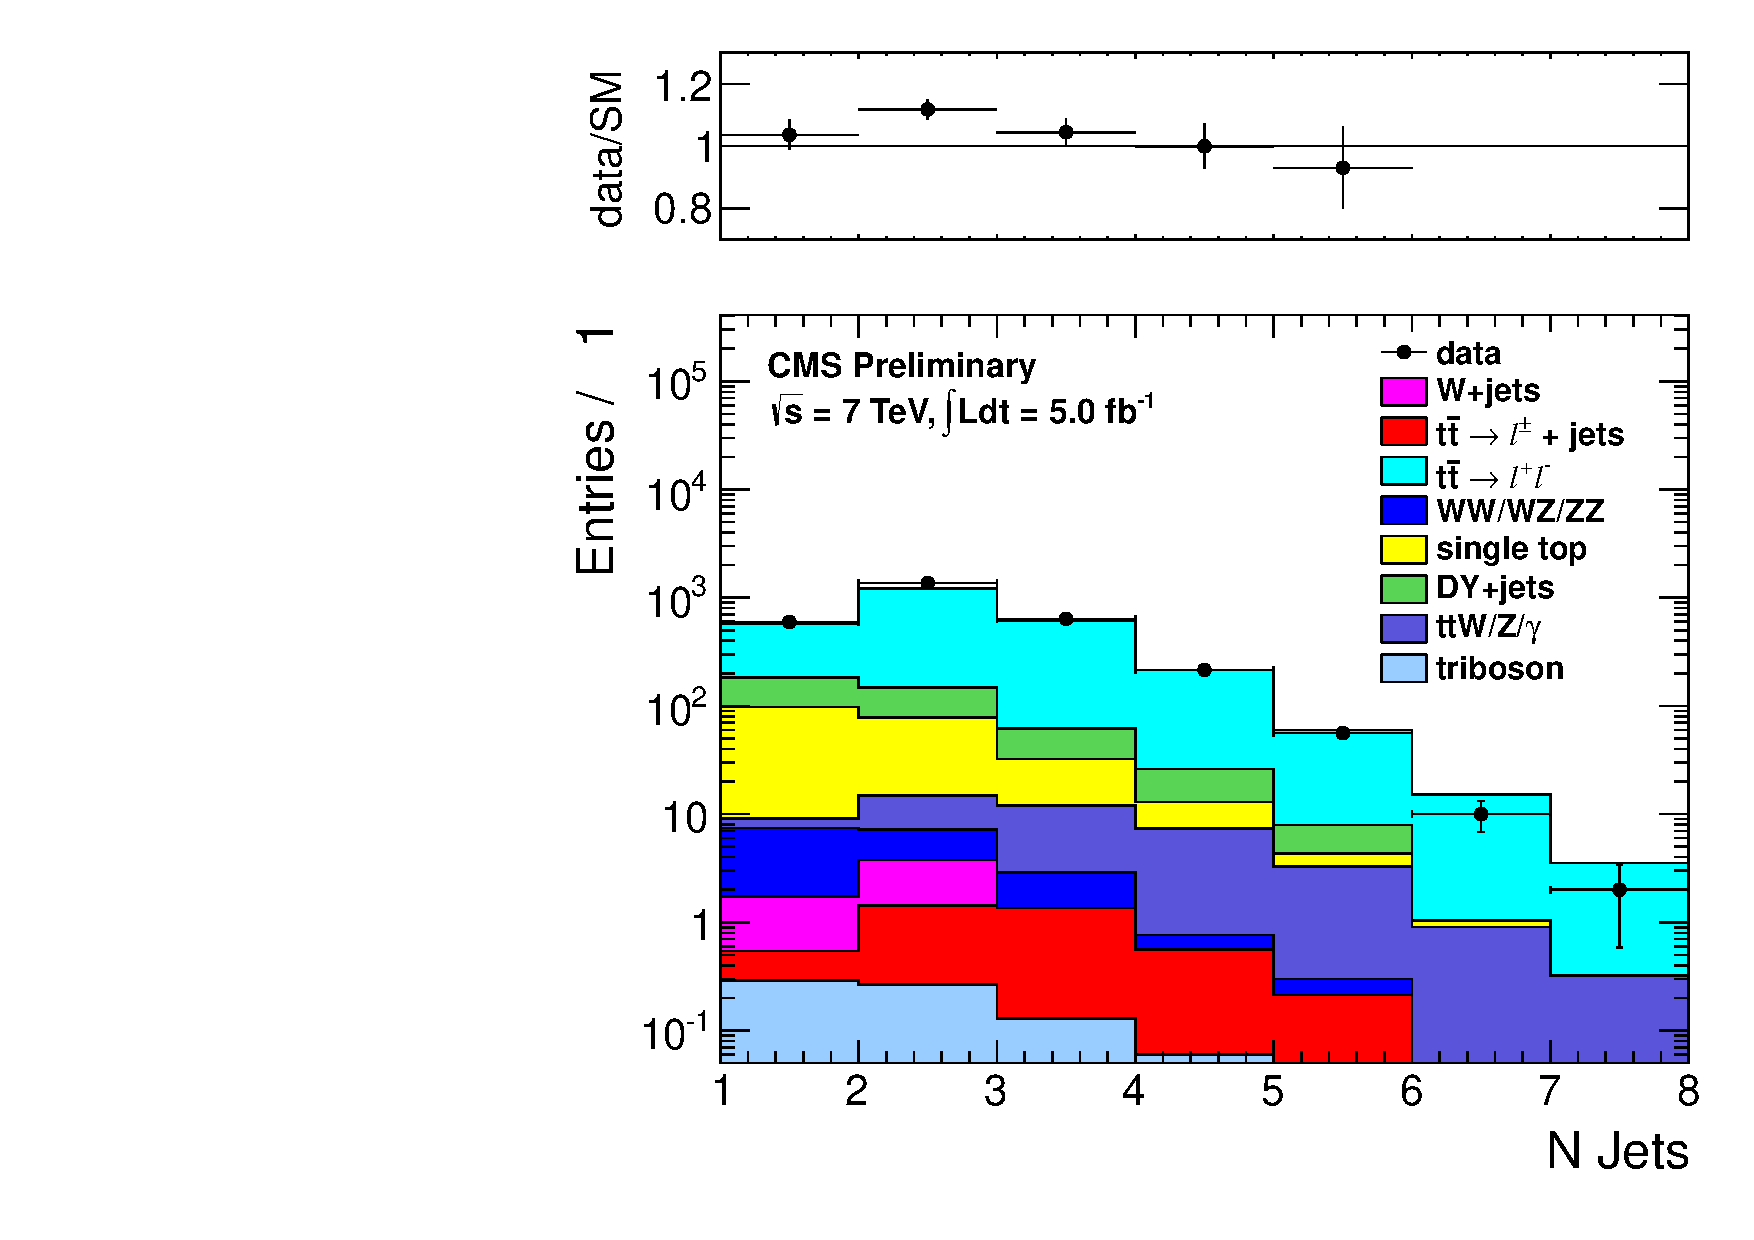
\includegraphics[width=0.5\linewidth]{plots/njets_all_dl_dimu.pdf}
	\caption{
	  \label{fig:dileptonnjets}%\protect 
          Comparison of the jet multiplicity distribution in data and MC for dilepton events in the \E-\M\
          (top), \E-\E\ (bottom left) and \M-\M\ (bottom right) channels.}  
      \end{center}
\end{figure}

It should be noted that in the case of \ttll\ events
with a single reconstructed lepton, the other lepton may be
mis-reconstructed as a jet. For example, a hadronic tau may be
mis-identified as a jet (since no $\tau$ identification is used). 
In this case only 1 additional jet from radiation may suffice for 
a \ttll\ event to enter the signal sample. As a result, both the
samples with $\ttbar+1$ jet and $\ttbar+\ge2$ jets are relevant for
the signal sample.

\begin{table}[!ht]
\begin{center}
\begin{tabular}{l|c}
\hline
            Jet Multiplicity Sample
            &                Data/MC Scale Factor \\
\hline
\hline
N jets $= 3$ (sensitive to $\ttbar+1$ extra jet from radiation)   &       $0.92 \pm 0.03$\\
N jets $\ge4$ (sensitive to $\ttbar+\ge2$ extra jets from radiation)   &       $0.83 \pm 0.04$\\
\hline
\end{tabular}
\caption{Data/MC scale factors used to account for differences in the
  fraction of events with additional hard jets from radiation in
  \ttll\ events. \label{tab:njetskfactors}}
\end{center}
\end{table}


\begin{figure}[hbt]
  \begin{center}
	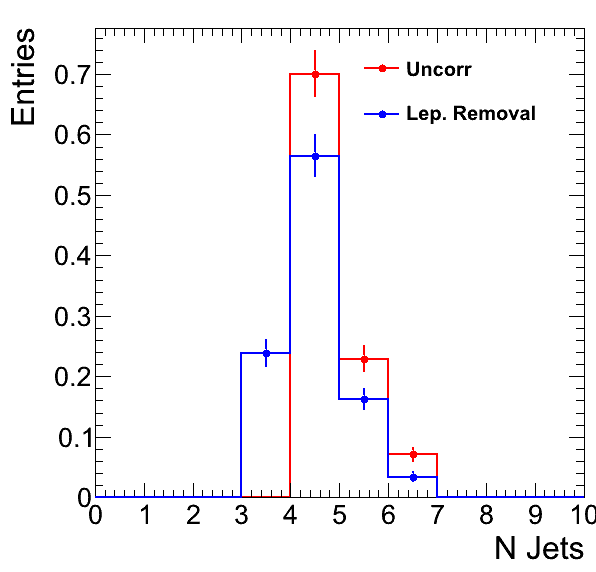
\includegraphics[width=0.5\linewidth]{plots/ttdl_njets_lepremoval_comp.png}
	\caption{
	  \label{fig:dileptonnjets_lepcomp}%\protect 
          Comparison of the jet multiplicity distribution for \ttll\
          events in MC in the signal sample before (red) and after
          (blue) applying the lepton-jet overlap removal. Note only
          the first 6 jets are shown.}  
      \end{center}
\end{figure}

Table.~\ref{tab:njetskfactors}  shows scale factors to correct the
fraction of events with additional jets in MC to the observed fraction
in data. These are applied to the \ttll\ MC in
the signal sample. In order to do so, it is first necessary to count the number of
additional jets from radiation and exclude leptons mis-identified as
jets. A jet is considered a mis-identified lepton if it is matched to a
generator-level second lepton with sufficient energy to satisfy the jet
\pt\ requirement ($\pt>30~\GeV$). 

In the signal sample, leptons mis-identified as jets are not rare. 
Figure~\ref{fig:dileptonnjets_lepcomp}  shows the MC jet
multiplicity distribution for \ttll\ events satisfying the full
selection criteria before and after subtracting leptons mis-identified
as jets. Approximately a quarter of the sample is comprised of 4-jet
events that actually correspond to a 2-lepton + 3 jet event where the second
lepton is counted as a jet. Lepton mis-identification depends strongly
on the type of second lepton, occuring more frequently in the case of
hadronic $\tau$s than leptonic objects. According to the \ttll\
MC, for hadronic $\tau$s, $\sim85\%$ of multi-prong $\tau$s and about half
the single-prong $\tau$ are mis-identified as jets. In the case of
leptonic objects, the fractions are smaller, comprising about a third
of \E/\M\ from a \W\ decay and $<20\%$ for leptonic $\tau$s, 
mainly because of the softness of the decay products. 
The scale factors listed in Table.~\ref{tab:njetskfactors} are applied
to the ``cleaned'' jet counts in the signal sample (shown in blue in
Figure~\ref{fig:dileptonnjets_lepcomp}). The impact of applying the
jet multiplicity scale factors on the \ttll\ is about a $10\%$ reduction in the
background prediction for the signal region. 

%\begin{itemize}
%\item Hadronic ($\tau$) objects: most multi-prong $\tau$s and about
%  half single-prong $\tau$s 
%\item Leptonic objects: smaller fraction, 
%\end{itemize}
%Fraction of various lepton types matched to a jet
%multi-prong taus ⟹ 85% give additional 30 GeV jet
%single-prong taus ⟹ ~50% give additional 30 GeV jet
%leptonic taus ⟹ <20% give additional 30 GeV jet
%e/mu⟹ ~40% give additional 30 GeV jet 

\begin{figure}[hbt]
  \begin{center}
	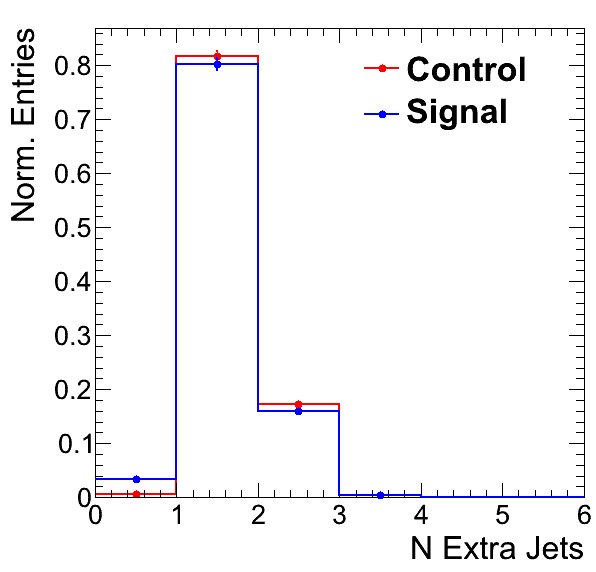
\includegraphics[width=0.5\linewidth]{plots/ttdl_njets_presel_3j_comp.png}%
	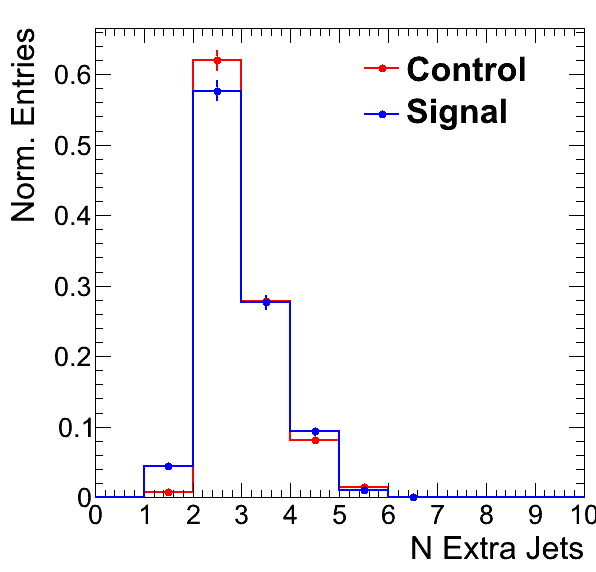
\includegraphics[width=0.5\linewidth]{plots/ttdl_njets_presel_4j_comp.png}
	\caption{
	  \label{fig:dileptonnjets_signalcontrol_comp}%\protect 
          Comparison of the number of additional jets from radiation
          in the 3-jet (left) and $\ge4$-jet (right) bins for the control \ttll\
          sample (with two reconstructed leptons) and the signal
          sample (with one reconstructed lepton). The distributions
          show good agreement, indicating that the usage of the
          reconstructed jet multiplicity in one sample to reweight the
        signal sample is indeed justified.}  
      \end{center}
\end{figure}

Ultimately, the interesting quantity for reweighting is the number of
additional hard jets from radiation and this information is accessed using the
number of reconstructed
jets. Figure~\ref{fig:dileptonnjets_signalcontrol_comp} 
demonstrates in MC that the \ttll control sample, i.e. when both leptons are reconstructed,
can indeed be used to reweight the \ttll signal sample, i.e. when one lepton is missed.
The figure compares the
number of additional jets from truth matching probed by N
reconstructed jets, in this case 3 and $\ge4$ jets. In order to do so,
jets that are truth-matched to the top decay products (the b-quarks
and additional leptons) are removed. The 3-jet distribution shows 
excellent agreement and the differences in the $\ge4$-jet distribution 
are at most $5\%$. The impact of possible differences in the
underlying distribution of extra
jets between the signal and control \ttll\ samples are estimated by
varying the scale factor contributions by $10\%$ and calculating the
change in the dilepton prediction. This effect is found to have a
negligible impact on the prediction, well below $1\%$.

Other effects that have been examined include the impact of 
additional jets from pileup that may bias the jet multiplicity
distribution, which  is found to be a negligible effect in this dataset. The
impact of the non-\ttll\ background on the jet fraction scale factors
has also been studied. In particular, given the large uncertainty on
the $\dy+HF$ MC prediction, this component has been varied by a factor
of 2 and the resulting change on the dilepton prediction is $<1\%$. As
a result, the dominant source of uncertainty is the statistical
uncertainty, primarily from the two-lepton control sample size, that
corresponds to a $3\%$ uncertainty on the dilepton prediction. 

The scale factors for the fraction of additional jets in the dilepton
sample are applied throughout the analysis. It may be noted that this
scaling is also performed consistently for the alternative \ttbar\
samples, always reweighting the jet multiplicity distribution to the
data in the \ttll\ control sample. In this way, effects truly
arising from using different MC samples and settings can be examined,
separately from issues related to the modeling of additional jets. 

\subsection{Normalization of the Top Prediction}

The overall normalization of the \ttbar\ sample is determined by
scaling to the \mt\ peak control region, following a procedure similar 
to that described in Section.~\ref{sec:bkg_singlelep}. This control
region is dominated by \ttbar\, albeit in its single lepton decay
mode. The basic idea is that after adjusting the modeling of
additional jets from radiation in the \ttll\ sample and correcting  
the leptonic branching fractions in the \ttbar\ sample, the MC 
prediction for the \ttlj\ and \ttll\ samples is subject to the same
sources of uncertainty: the \ttbar\ cross section, the luminosity, the
selection efficiencies, etc$\dots$ The exception is the veto on events
containing an isolated track, since this last requirement has a different 
impact on the \ttlj\ and \ttll\ samples. The impact of this
requirement is addressed separately in Section.~\ref{sec:trkveto}. 

The \mt-peak scale factor is thus determined after applying the full
analysis selection with the exception of the isolated track veto. 
Specifically, the pre-veto sample is defined by the following requirements
\begin{itemize}
\item At least 1 selected electron (muon) with \pt $>$ 30 GeV and $|\eta|<2.5$ ($|\eta|<2.1$)
\item At least 4 selected jets, of which at least 1 is b-tagged
\item \met\ $>$ 50 GeV
\end{itemize}

As in the case of the single lepton + jets sample, scaling the overall 
normalization to the \mt\ peak largely reduces the dependence on the
\ttbar\ cross section and cancels systematic uncertainties associated
with effects such as the luminosity, selection efficiencies,
etc$\dots$ However, the \mt\ peak control sample is contaminated 
by non-\ttbar\ processes, particularly \wjets\ that contributes at
the $5-10\%$ level, even after requiring a b-tagged jet. The \wjets+HF
process is a particular concern given the large theoretical
uncertainties associated with their production. 
Therefore a systematic uncertainty is derived to account for
the uncertainty in this background component. The normalization of 
the \wjets\ sample is scaled up and down by $50\%$ and the full 
background estimate recomputed. The impact of such a variation on 
the dilepton sample is of $~5\%$, as shown in 
Table.~\ref{tab:samplecomposition}. However, since the
single lepton + jets prediction decreases because of the large
variation in the \wjets\ component, the impact on the total background
prediction is significantly smaller, at the level of $\sim 1\%$.

\begin{table}
\begin{center}
\begin{tabular}{l|c|c|c}
\hline
	Sample 	& Nominal	& W+Jets x1.5		& W+Jets x0.5\\
\hline
\hline
$t\bar{t} \rightarrow l^{+}l^{-} $ 	 & 	 85.0 $\pm$ 3.8 (4 \%)			 & 	 81.4 $\pm$ 3.7			 & 	 89.0 $\pm$ 3.8 \\  
$t\bar{t} \rightarrow l^{\pm} $+ jets 	 & 	 12.3 $\pm$ 0.6 (5 \%) 			 & 	 11.7 $\pm$ 0.6  		 & 	 12.8 $\pm$ 0.6 \\  
W+jets 	 & 	 7.6 $\pm$ 3.9 (51 \%) 							 & 	 10.9 $\pm$ 5.5  		 & 	 4.0 $\pm$ 2.0 \\   
single top 	 & 	 5.7 $\pm$ 0.6 (11 \%) 						 & 	 5.4 $\pm$ 0.6   		 & 	 5.9 $\pm$ 0.7 \\   
WW/WZ/ZZ 	 & 	 0.5 $\pm$ 0.2 (33 \%) 						 & 	 0.5 $\pm$ 0.2   		 & 	 0.6 $\pm$ 0.2 \\   
%DY+jets 	 & 	 0.0 $\pm$ 0.0 (0 \%) 						 & 	 0.0 $\pm$ 0.0   		 & 	 0.0 $\pm$ 0.0 \\   
ttW/Z/$\gamma$ 	 & 	 5.6 $\pm$ 0.4 (7 \%) 						 & 	 5.4 $\pm$ 0.4   		 & 	 5.9 $\pm$ 0.4 \\   
triboson 	 & 	 0.1 $\pm$ 0.0 (40 \%) 						 & 	 0.1 $\pm$ 0.0   		 & 	 0.1 $\pm$ 0.0 \\   
\hline
Total 	 & 	 116.8 $\pm$ 5.5 (5 \%)						 & 	 115.5 $\pm$ 6.7 (6 \%)	& 	 118.2 $\pm$ 4.4 (4 \%) \\
\hline
Non-tt dilepton 	 & 	 31.8 $\pm$ 4.0 (12 \%)				& 	 34.0 $\pm$ 5.6 (16 \%)		& 	 29.3 $\pm$ 2.2 (8 \%) \\
\hline
\hline
Data/MC ctr SF &	0.90 $\pm$ 0.03	& 0.86 $\pm$ 0.03	&	0.94 $\pm$ 0.03 \\
\hline
MC sig/ctr SF &		0.079 $\pm$ 0.003	& 0.078 $\pm$ 0.004	&	0.080 $\pm$ 0.002 \\
\hline
\end{tabular}
\caption{Comparison of the nominal background predictions and those
  under the assumption that the \wjets\ normalization is 50\%
  higher and $50\%$ lower than the nominal. NUMBERS TO BE UPDATED 
  \label{tab:samplecomposition}%\protect
}  
\end{center}
\end{table}

It should be noted that the background prediction obtained using
the same normalization scale factor based on the \mt\ peak for the 
single lepton and dilepton samples is subject to smaller uncertainties
than the prediction obtained by normalizing the \ttll\ component alone
to the overall yield in the two-lepton control sample. The reason is 
that the normalization of the two-lepton control yield depends on
effects that do not impact the \ttll\ sample with one reconstructed
lepton (i.e. the signal sample of interest) in the same way. Example
of these effects include the dilepton trigger and second lepton
reconstruction efficiencies.

In conclusion, the pre-veto sample is used to define an overall data
over MC scale factor ($SF^{\rm{all}}$) in the \mt\ peak control region, that is
applied to all background predictions and is simply defined as
\begin{itemize}
\item $N_{\rm{peak}}^{\rm{all}}$ = data yield in the peak region $60<\mt<100$ GeV
\item $M_{\rm{peak}}^{\rm{all}}$ = MC yield in the peak region $60<\mt<100$ GeV
\item $SF^{\rm{all}} = N_{\rm{peak}}^{\rm{all}} / M_{\rm{peak}}^{\rm{all}}$
\end{itemize}
For all subsequent steps, the scale factor $SF^{\rm{all}}$ is applied to all MC contributions.

\subsection{The Isolated Track Veto}
\label{sec:trkveto}

The \ttll\ background is further suppressed after the $4$-jet
requirement by removing events with any non-isolated track with 
$\pt>10~\GeV$. The isolated track veto rejects events with an 
\E\ or a \M, as well as single-prong $\tau$-decays. 
This veto is very effective at reducing the dilepton background. In
particular, according to the \ttll\ MC, the veto removes about
three-quarters of events with an \E\ or \M\ from the \W\ decay and
almost half the leptonic and single prong $\tau$
decays. The veto has no impact on multi-prong $\tau$s, though this is
a smaller component overall. Since the \ttll\ background includes
different types of processes, it is useful to first characterize the
composition of this background. 

\subsubsection{Top Dilepton Sample Composition}

The \ttll\ background may be categorized based on the type of
second lepton, as shown in Table.~\ref{tab:ttdlcomposition}. The main
component is from electrons and muons from a \W\ decay or through an
intermediate $\tau$ decay. The second largest component arises from
single-prong hadronic $\tau$ decays, followed by multi-prong
$\tau$s. Finally an additional contribution arises from leptons
falling in the forward region, outside the Tracker acceptance
$|\eta|>2.5$ (refered to as `lost').

\begin{table}[!ht]
\begin{center}
\begin{tabular}{l|c|c}
\hline
            Sample					&                Yield   & 	Fraction [\%]\\
\hline
\hline
$t\bar{t} \rightarrow l^{+}l^{-} (\mathrm{lost})$   &       7 $\pm$ 1 	& 	6\\
$t\bar{t} \rightarrow l^{+}l^{-} (e/\mu)$   &      30 $\pm$ 3  	& 26\\
$t\bar{t} \rightarrow l^{+}l^{-} (\tau_{\mathrm{lep}})$   &      21 $\pm$ 2  	& 18\\
$t\bar{t} \rightarrow l^{+}l^{-} (\tau_{\mathrm{had}}\rightarrow \mathrm{1-prong})$   &      39 $\pm$ 3  & 34\\
$t\bar{t} \rightarrow l^{+}l^{-} (\tau_{\mathrm{had}}\rightarrow \mathrm{3-prong})$   &      19 $\pm$ 2  & 16\\
\hline
         total $t\bar{t} \rightarrow l^{+}l^{-} $  &     117 $\pm$ 5  & 100\\
\hline
\end{tabular}
\caption{Dilepton events satisfying the full selection criteria
 and \met\ $>$ 100 GeV, \mt\ $>$ 150 GeV,  separated by decay modes.
Recall that \ttll\ accounts for $\approx80$\% of the total background.
\label{tab:ttdlcomposition}}
\end{center}
\end{table}

The isolated track veto does not apply to the components where the
second lepton falls outside the acceptance or where it decays to a 
hadronic tau that is not explicitly rejected. For the cases where the
second lepton includes an electron or muon or a charged $\pi/K$, it is
possible to further distinguish cases when the relevant particle
targeted by the veto is below the \pt\ threshold. Matching the
truth-level particle to reconstructed tracks shows that in \ttll\ MC
\begin{itemize}
\item for $t\bar{t} \rightarrow l^{+}l^{-} (e/\mu)$, about a third of
  the sample falls below the \pt\ threshold of the track veto, and the remaining 
  two thirds fail the isolation
\item for $t\bar{t} \rightarrow l^{+}l^{-} (\tau_{\mathrm{lep}})$,
  about $80\%$ are soft $\pt<10~\GeV$ and about $20\%$ are
  non-isolated
\item for $t\bar{t} \rightarrow l^{+}l^{-}
  (\tau_{\mathrm{had}}\rightarrow \mathrm{1-prong})$, 
about $70\%$ are soft, as expected from a $\tau$ decay product and the
rest fail the isolation criteria.
\end{itemize}
In summary, the combination of these fractions with the relative sample
composition listed in Table.~\ref{tab:ttdlcomposition} shows that only
about a third of the \ttll\ background sample is from 2nd leptons (e, $\mu$, or $\tau\to$1-prong)
which satisfy \pt\ $>$ 10 GeV but fail the track isolation criterion
veto\footnote{Explicitly, the fraction of events that give rise to a
  sufficiently energetic lepton or single prong $\tau$ is: $70\%$ of \E-\M\ events
  which are $26\%$ of the sample, $20\%$ of leptonic tau events which
  are $18\%$ of the sample and $30\%$ of single prong $\tau$ events 
  which are $10\%$ of the sample.}. The performance of the isolation
used in the track veto requirement is the subject of the next section.

It should also be noted that according to the MC, track reconstruction 
inefficiencies affect a few percent ($\sim 1-2\%$) of the
leptonic and single prong $\tau$ events. The tracking efficiency in
this analysis is taken from MC, which is expected to provide good modeling of isolated 
tracks with $\pt>10~\GeV$. The impact of  
possible differences between data and MC is found to be negligible. 
In particular, the case of single-prong taus is the most challenging to
model due to the effect of nuclear interactions in the tracker material. 
Past studies of the tracking efficiency for pions~\cite{TRK10002}
provide a data/MC uncertainty in the tracking efficiency of $3.9\%$\footnote{
This tracking efficiency uncertainty estimate is conservative for this 
analysis since it includes tracks of \pt\ down to $250$ MeV, where
material effects are larger and so are the corresponding
uncertainties.}. Propagating this uncertainty to the total background
estimate yields a total uncertainty of $< 0.5\%$. The reason is that
the tracking efficiency uncertainty only applies to single prong
$\tau$ decays with $\pt> 10~\GeV$, which are under $30\%$ of the 
dilepton component, which in turn is $\sim 80\%$ of the total sample.  

To conclude, the \ttll\ background arises from events where the second
lepton falls outside the acceptance (both in $\eta$ and $\pt$),
because the event contains a hadronic tau that is not explicitly rejected or
because the second lepton fails the isolation requirement. 
Even though the \ttll\ sample is quite heterogenous and comprises
multiple types of second lepton events, there are two
main sources of uncertainty in this estimate: 
\begin{itemize}
\item Acceptance effects, which are estimated by using alternative MC
  samples
\item Detector effects, mainly arising from understanding the
  performance of the isolated track veto, which impacts only about a
  third of the total \ttll\ sample.
\end{itemize}

\subsubsection{Performance of the Isolation Requirement}

The last requirement used in the analysis is an isolated track
veto. This selection criteria rejects events containing a track of $\pt>10~\GeV$
with relative track isolation $\sum \pt/\pt(trk)$ in a cone of size $R=0.3<0.1$. It may be noted that only tracks consistent with the
vertex with highest $\sum \pt^2$ are considered in order to
reduce the impact of spurious tracks, for example from pileup interactions. This requirement has very good
performance. Figure~\ref{fig:isolvetoroc} shows the
efficiency for rejecting dilepton events compared to the efficiency
for selecting single lepton events for various cone sizes and cut
values. The chosen working point provides a signal efficiency of
$\epsilon(sig) =92\%$ for a background rejection of $\epsilon(bkg)
=53\%$ in MC. 

\begin{figure}[hbt]
  \begin{center}
	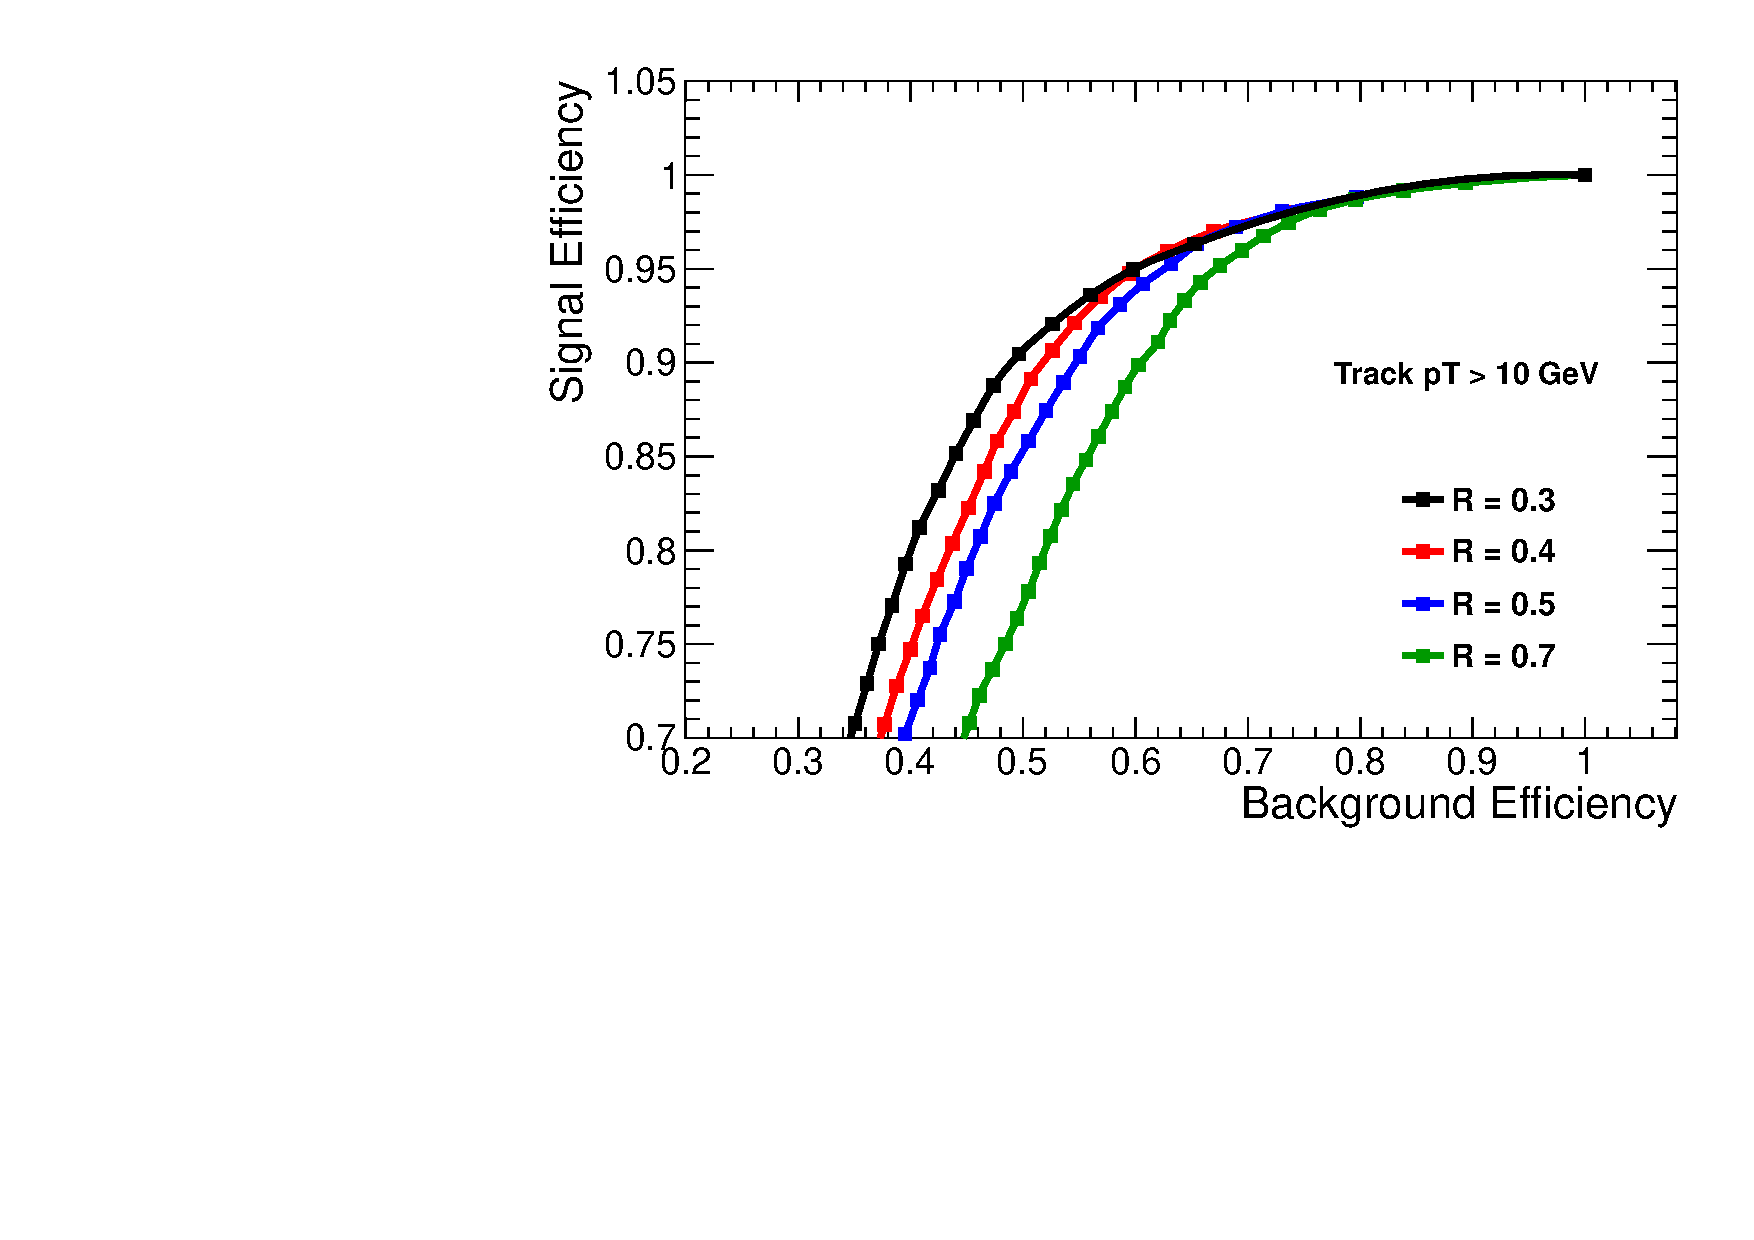
\includegraphics[width=0.7\linewidth]{plots/roc_ttdl_trkiso_pt10.pdf}
	\caption{
	  \label{fig:isolvetoroc}%\protect 
          Comparison of the performance in terms of signal (single lepton events) efficiency
         and background (dilepton events) rejection for various cone
         sizes and cut values. The current isolation requirement uses
         a cone of size $\Delta R = 0.3$ and a cut value of 0.1,
         corresponding to $\epsilon(sig) =92\%$ for $\epsilon(bkg)=53\%$.
       ADD ARROW OR LINE TO INDICATE WORKING POINT.}  
      \end{center}
\end{figure}

It should be emphasized that the isolated track veto has a different impact on the samples with a single
lepton (mainly \ttlj\ and \wjets) and that with two leptons (mainly \ttll).
For the dilepton background, the veto rejects events which have a
genuine second lepton. Thus the performance may be understood
as an efficiency $\epsilon(trk)$ to identify the isolated track. In the
case of the single lepton background, the veto rejects events
which do not have a genuine second lepton, but rather which contain 
a ``fake'' isolated track. The isolated track veto thus effectively scales the
single lepton sample by (1-FR), where FR is the ``fake rate'' to 
identify an isolated track in events which contain no genuine second
lepton. It is thus necessary to study the isolated track efficiency
$\epsilon(trk)$ and the ``fake rate'' FR in order to fully
characterize the veto performance. 

The veto efficiency for dilepton events is calculated using 
the tag and probe method in \Z\ events. A good lepton
satisfying the full ID and isolation criteria and matched to a
trigger object serves as the tag. The probe is defined as a track with
$\pt>10~\GeV$ that has opposite charge to the tag and has an invariant
mass with the probe consistent with the \Z\ mass. 

The variable used to study the performance of the veto is the absolute track isolation,
since it removes the dependence of the isolation variable on the \pt\ of the
object under consideration. This is particularly useful because the
underlying \pt\ distribution is different for second leptons in
\ttll\ events compared to \Z\ events, particularly due to the presence of $\tau$s
that have softer decay products. As shown in Figure~\ref{fig:absiso}, the absolute
isolation is consistent between $\Z+4$ jet events and \ttll\ events,
including leptons from \W\ and $\tau$ decays. This supports the notion
that the isolation, defined as the energy surrounding the object under
consideration, depends only on the environment of the object and not
on the object itself. The isolation is thus sensitive to the ambient
pileup and jet activity in the event, which is uncorrelated with
the lepton \pt. It is thus justified to use tag and probe in
$\Z+4$ jet events, where the jet activity is similar to \ttll\
events in our \njets\ $>$ 4 signal region, in order to estimate the performance of the isolation 
requirement for the various leptonic categories of \ttll\ events. 

\begin{figure}[hbt]
  \begin{center}
	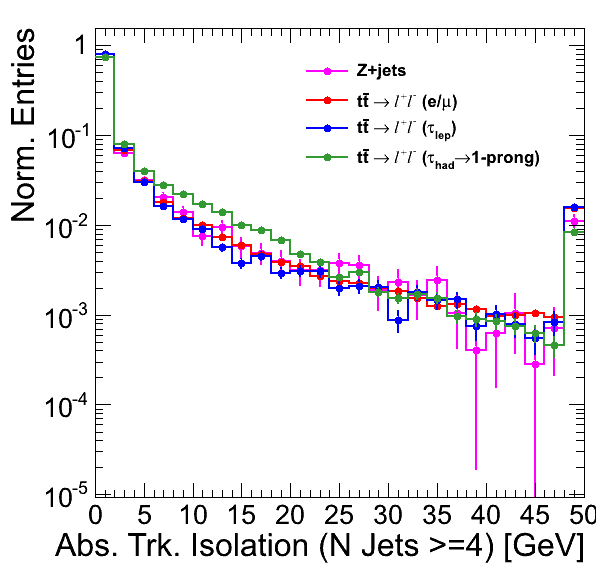
\includegraphics[width=0.5\linewidth]{plots/pfabsiso_njets4_log.png}%
	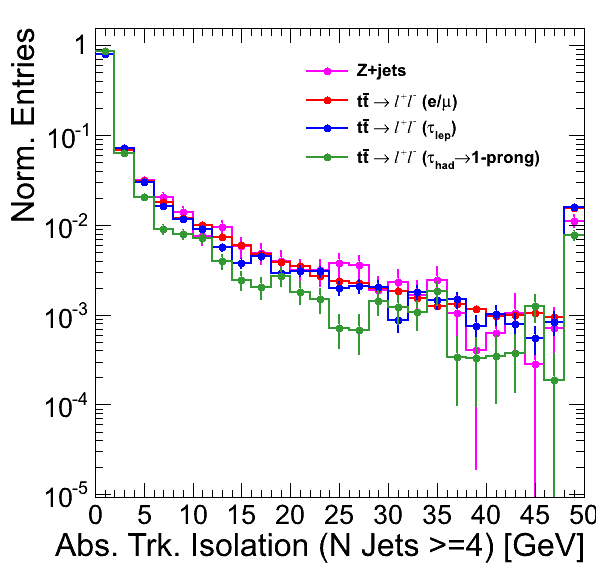
\includegraphics[width=0.5\linewidth]{plots/pfabsiso_njets4_clean_log.png}
	\caption{
	  \label{fig:absiso}%\protect 
          Comparison of absolute track isolation for track probes in
          $\Z+4$ jet and \ttll\ events for different lepton types. The
          isolation variables agree across samples, except for single
          prong $\tau$s, that tend to be slightly less isolated
          (left). The agreement across isolation distributions is
          recovered after removing single prong $\tau$ events produced 
          in association with $\pi^0$s from the sample (right).}  
      \end{center}
\end{figure}

It may be noted that tracks from single prong $\tau$ decays are
slightly less isolated compared to electrons and muons. The reason is that single
prong $\tau$s can have $\pi^0$ associated with the single charged
track. These decay into $\gamma$s that in turn convert $\gamma\to e^+e^-$ and spoil the
isolation. As also shown in Figure~\ref{fig:absiso},
the isolation distribution for charged tracks from $\tau$ decays that
are not produced in association with $\pi^0$s are consistent with that
from $\E$s and $\M$s. Since events from single prong
$\tau$ decays produced in association with $\pi^0$s comprise a small
fraction of the total sample, the isolation measured for leptons is used
for all single prong $\tau$ events. A systematic uncertainty is
assigned to account for the difference in the underlying
isolation distribution for this sample.

%Figure.~\ref{fig:reliso} compares the relative track isolation
%for events with a track with $\pt > 10~\GeV$ in addition to a selected
%muon for $\Z+4$ jet events and various \ttll\ components. The
%isolation distributions show significant differences, particularly
%between the leptons from a \W\ or \Z\ decay and the tracks arising
%from $\tau$ decays. As can also be seen in the figure, the \pt\
%distribution for the various categories of tracks is different, where
%the decay products from $\tau$s are significantly softer. Since the
%\pt\ enters the denominator of the isolation definition and hence
%alters the isolation variable...

%\begin{figure}[hbt]
%  \begin{center}
%	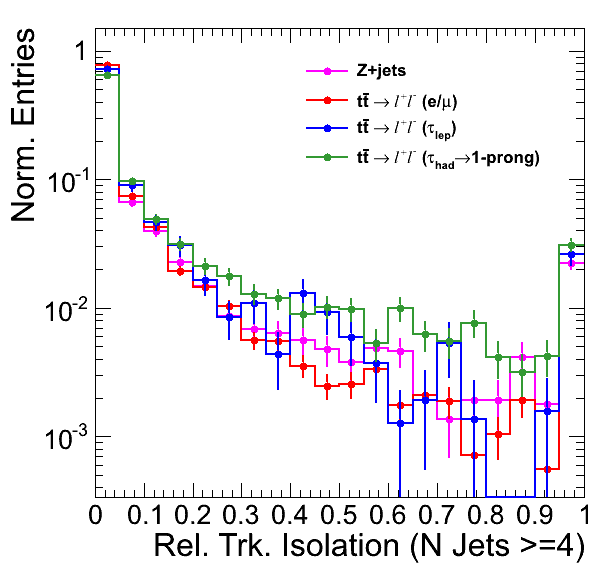
\includegraphics[width=0.5\linewidth]{plots/pfiso_njets4_log.png}%
%	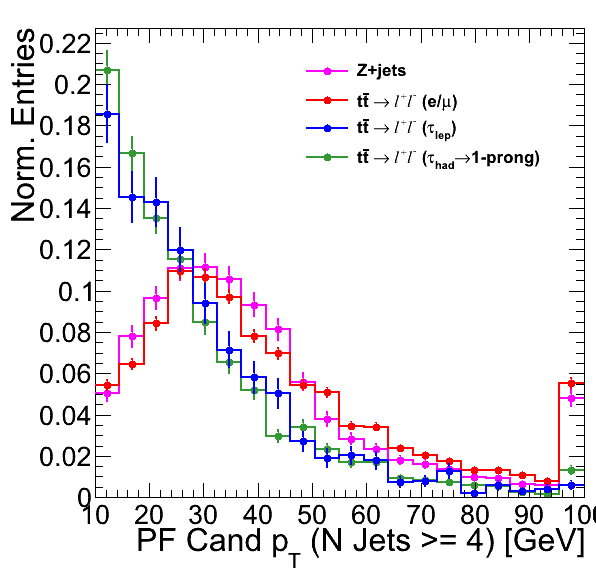
\includegraphics[width=0.5\linewidth]{plots/pfpt_njets4.png}
%	\caption{
%	  \label{fig:reliso}%\protect 
%          Comparison of relative track isolation variable for PF cand probe in Z+jets and ttbar 
%          Z+Jets and ttbar dilepton have similar isolation distributions
%          ttbar with leptonic and single prong taus tend to be less
%          isolated. The difference in the isolation can be attributed
%          to the different \pt\ distribution of the samples, since
%          $\tau$ decay products tend to be softer than leptons arising
%          from \W\ or \Z\ decays.}  
%      \end{center}
%\end{figure}

%	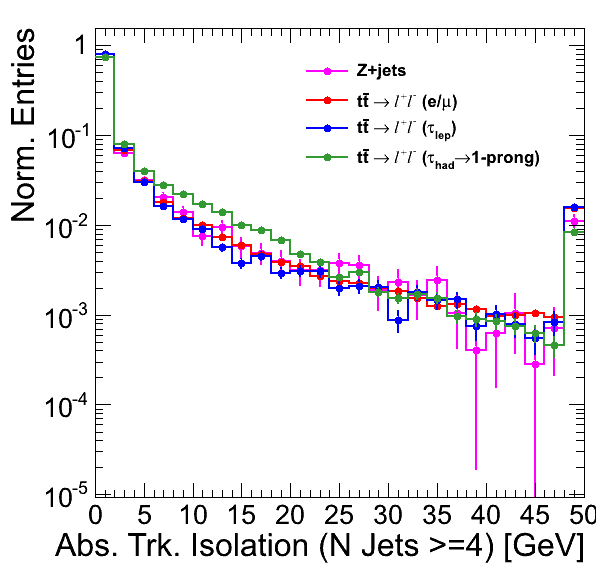
\includegraphics[width=0.5\linewidth]{plots/pfabsiso_njets4_log.png}


%BEGIN SECTION TO WRITE OUT 
%In detail, the procedure to correct the dilepton background is:

%\begin{itemize}
%\item Using tag-and-probe studies, we plot the distribution of {\bf absolute} track isolation for identified probe electrons
%and muons {\bf TODO: need to compare the e vs. $\mu$ track iso distributions, they might differ due to e$\to$e$\gamma$}.
%\item We verify that the distribution of absolute track isolation does not depend on the \pt\ of the probe lepton.
%This is due to the fact that this isolation is from ambient PU and jet activity in the event, which is uncorrelated with
%the lepton \pt {\bf TODO: verify this in data and MC.}.
%\item Our requirement is {\bf relative} track isolation $<$ 0.1. For a given \ttll\ MC event, we determine the \pt of the 2nd
%lepton and translate this to find the corresponding requirement on the {\bf absolute} track isolation, which is simply $0.1\times$\pt.
%\item We measure the efficiency to satisfy this requirement in data and MC, and define a scale-factor $SF_{\epsilon(trk)}$ which
%is the ratio of the data-to-MC efficiencies. This scale-factor is applied to the \ttll\ MC event.
%\item {\bf THING 2 we are unsure about: we can measure this SF for electrons and for muons, but we can't measure it for hadronic 
%tracks from $\tau$ decays. Verena has showed that the absolute track isolation distribution in hadronic $\tau$ tracks is harder due 
%to $\pi^0\to\gamma\gamma$ with $\gamma\to e^+e^-$.}
%\end{itemize} 
%END SECTION TO WRITE OUT 


A measurement of the FR in data is non-trivial. However, it is
possible to correct for differences in the FR between data and MC by
applying an additional scale factor for the single lepton background
alone, using the sample in the \mt\ peak region. This scale factor is determined after applying the isolated track
veto and after subtracting the \ttll\ component, corrected for the
isolation efficiency derived previously. 
As shown in Figure~\ref{fig:vetoeffcomp}, the efficiency for selecting an
isolated track in single lepton events is independent of \mt\, so the use of
an overall scale factor is justified to estimate the contribution in
the \mt\ tail. 

\begin{figure}[hbt]
  \begin{center}
	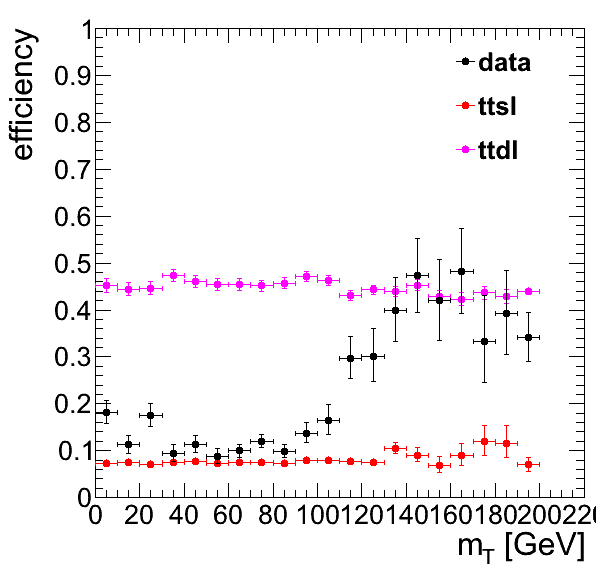
\includegraphics[width=0.5\linewidth]{plots/vetoeff_comp.png}
	\caption{
	  \label{fig:vetoeffcomp}%\protect 
          Efficiency for selecting an isolated track comparing
          single lepton \ttlj\ and dilepton \ttll\ events in MC and 
          data as a function of \mt. The
          efficiencies in \ttlj\ and \ttll\ exhibit no dependence on
          \mt\, while the data ranges between the two. This behavior
          is expected since the low \mt\ region is predominantly \ttlj, while the
          high \mt\ region contains mostly \ttll\ events.}  
      \end{center}
\end{figure}


\section{Summary of the Background Estimation Procedure}

The SM background in the signal region, defined by requirements of
large \met\ and \mt, is estimated using MC. The MC is validated using
data control samples, which are used to derive data-to-MC scale 
factors and corresponding uncertainties.

The procedure to estimate the background prediction may be summarized
as
\begin{itemize}
\item Apply the state-of-the-art corrections to the MC, reflecting the
  best knowlege of the detector performance, in order to improve the agreement
  with the data. This includes effects such as the modeling of the pileup, the jet energy scale,
  \met\ corrections, etc$\dots$ 
\item Correct the leptonic branching fractions in the \ttbar\ MC
\item Use the dilepton sample with two selected leptons to reweight
  the \njets\ distribution in \ttll\ MC, which is not necessarily
  well-modeled due to the presence of additional jets from radiation.
\item Use the pre-veto sample (i.e. applying the full analysis selection
  with the exception of the isolated track veto) to define a scale
  factor in the \mt\ peak region. This scale factor corrects for
  effects of integrated luminosity, \ttbar\ cross section, lepton
  selection and trigger efficiencies.
\item Correct the \ttll\ sample for differences between data and MC in the isolation for
  events with a second lepton. This correction is derived using $\Z+4$
  jet events and applied to the \ttll\ sample. 
\item In the signal sample, after applying the full selection
  including the isolated track veto, derive a scale factor to
  account for possible data vs. MC discrepancies in the isolated track 
  fake rate for backgrounds which have a single genuine lepton. This
  scale factor is applied to the single lepton backgrounds only.
\end{itemize}

%We consider three samples:
%
%\begin{itemize}
%\item Dilepton sample (exactly 2 selected leptons): used to correct the \njets\ distribution in \ttll\ MC, which is not necessarily well-modelled since ISR jets 
%are needed to satisfy the \njets $\geq$ 4 requirement defining the signal region;
%\item Inclusive sample (at least 1 selected lepton): used to define a
%  scale factor which corrects for effects of integrated luminosity,
%  \ttbar\ cross section, jet energy scale and jet selection efficiencies, lepton selection and trigger efficiencies.
%\item Signal sample (exactly 1 selected lepton): this is the sample used to define the signal region. In addition, this sample is used to determine a scale 
%factor accounting for possible data vs. MC discrepancies in the isolated track fake rate for backgrounds which have only 1 genuine lepton.
%\end{itemize}
%
%\subsection{Step 1: Use dilepton control sample to correct the \njets\ distributon in \ttll\ MC}
%
%The dilepton control sample is defined by the following requirements:
%\begin{itemize}
%\item Exactly 2 selected electrons or muons with \pt $>$ 20 GeV
%\item \met\ $>$ 50 GeV
%\item $\geq1$ b-tagged jet
%\end{itemize}
%
%This sample is dominated by \ttll. The distribution of \njets\ for data and MC passing this selection is displayed in Fig.~\ref{fig:dilepton_njets}. 
%We use this distribution to derive scale factors which reweight the \ttll\ MC \njets\ distribution to match the data. We define the following
%quantities
%
%\begin{itemize}
%\item $N_{2}=$ data yield minus non-dilepton \ttbar\ MC yield for \njets\ $\leq$ 2
%\item $N_{3}=$ data yield minus non-dilepton \ttbar\ MC yield for \njets\ = 3
%\item $N_{4}=$ data yield minus non-dilepton \ttbar\ MC yield for \njets\ $\geq$ 4
%\item $M_{2}=$ dilepton \ttbar\ MC yield for \njets\ $\leq$ 2
%\item $M_{3}=$ dilepton \ttbar\ MC yield for \njets\ = 3
%\item $M_{4}=$ dilepton \ttbar\ MC yield for \njets\ $\geq$ 4
%\end{itemize}
%
%We use these yields to define 3 scale factors, which quantify the data/MC ratio in the 3 \njets\ bins:
%
%\begin{itemize}
%\item $SF_2 = N_2 / M_2$
%\item $SF_3 = N_3 / M_3$
%\item $SF_4 = N_4 / M_4$
%\end{itemize}
%
%And finally, we define the scale factors $K_3$ and $K_4$:
%
%\begin{itemize}
%\item $K_3 = SF_3 / SF_2$
%\item $K_4 = SF_4 / SF_2$
%\end{itemize}
%
%The scale factor $K_3$ is extracted from dilepton \ttbar\ events with \njets = 3, which have exactly 1 ISR jet.
%The scale factor $K_4$ is extracted from dilepton \ttbar\ events with \njets $\geq$ 4, which have at least 2 ISR jets.
%Both of these scale factors are needed since dilepton \ttbar\ events which fall in our signal region (including
%the \njets $\geq$ 4 requirement) may require exactly 1 ISR jet, in the case that the second lepton is reconstructed
%as a jet, or at least 2 ISR jets, in the case that the second lepton is not reconstructed as a jet. These scale
%factors are applied to the dilepton \ttbar\ MC only. For a given MC event, we determine whether to use $K_3$ or $K_4$
%by counting the number of reconstructed jets in the event ($N_{\rm{jets}}^R$) , and subtracting off any reconstructed 
%jet which is matched to the second lepton at generator level ($N_{\rm{jets}}^\ell$); $N_{\rm{jets}}^{\rm{cor}} = N_{\rm{jets}}^R - N_{\rm{jets}}^\ell$.
%For events with $N_{\rm{jets}}^{\rm{cor}}=3$ the factor $K_3$ is applied, while for events with $N_{\rm{jets}}^{\rm{cor}}\geq4$ the factor $K_4$ is applied.
%For all subsequent steps, the scale factors $K_3$ and $K_4$ have been applied to the \ttll\ MC.
% 
%\subsection{Step 2: Use the pre-veto sample to define a data-to-MC scale factor}
%
%The pre-veto sample is defined by the following requirements
%
%\begin{itemize}
%\item At least 1 selected electron (muon) with \pt $>$ 30 GeV and $|\eta|<2.5$ ($|\eta|<2.1$)
%\item At least 4 selected jets, with at least 1 b-tagged jet
%\item \met\ $>$ 50 GeV
%\end{itemize}
%
%Thus all selection criteria are applied with the exception of the veto on events containing an isolated track. 
%This sample is dominated by \ttlj\, with secondary contributions from \wjets\ and \ttll\ . 
%%The largest contribution to this sample is \ttlj, but \wjets\ and \ttll\ also have significant contributions.
%This sample is used to define an overall data over MC scale factor ($SF$) in the peak control region, 
%that accounts for differences between the data and the MC due to the luminosity estimate, the lepton 
%efficiencies and so on and is thus applied to the full MC cocktail. 
%To do so we define for the pre-veto sample (labeled `all'):
%
%\begin{itemize}
%\item $N_{\rm{peak}}^{\rm{all}}$ = data yield in the peak region $60<\mt<100$ GeV
%\item $M_{\rm{peak}}^{\rm{all}}$ = MC yield in the peak region $60<\mt<100$ GeV
%\item $SF^{\rm{all}} = N_{\rm{peak}}^{\rm{all}} / M_{\rm{peak}}^{\rm{all}}$
%\end{itemize}
%
%For all subsequent steps, the scale factor $SF^{\rm{all}}$ is applied to all MC contributions.
%
%\subsection{Step 3: Isolated Track Veto Efficiency Correction}
%
%The signal sample is defined by the same requirements as the pre-veto sample, except that we veto events containing
%an isolated track. The background is the inclusive sample can be split into 2 contributions:
%
%\begin{itemize}
%\item Dilepton background: mostly \ttll.
%\item Single lepton background: mostly \ttlj\ and \wjets;
%\end{itemize}
%
%The isolated track veto impacts these 2 contributions in different ways. For the dilepton background, the veto
%rejects events which have a genuine 2nd lepton, so applying the isolated track veto scales the dilepton background
%by the efficiency $\epsilon(trk)$ to identify the isolated track. For the single lepton background, the veto rejects events
%which do not have a genuine 2nd lepton but which have a ``fake'' isolated track, so the isolated track veto scales
%the single lepton background by (1-FR), where FR is the ``fake rate'' to identify an isolated track in events which 
%contain no genuine 2nd lepton. 
%
%The isolated track efficiency $\epsilon$ can be measured in data and MC using $Z\to\ell\ell$ tag-and-probe studies. 
%We therefore use the tag-and-probe studies to apply a correction to the \ttll\ MC. 
%A measurement of the FR in data is non-trivial, but we can account for differences between the data and the MC by scaling 
%only the single lepton background in the \mt\ peak region after applying the isolated track veto.
%
%In detail, the procedure to correct the dilepton background is:
%
%\begin{itemize}
%\item Using tag-and-probe studies, we plot the distribution of {\bf absolute} track isolation for identified probe electrons
%and muons {\bf TODO: need to compare the e vs. $\mu$ track iso distributions, they might differ due to e$\to$e$\gamma$}.
%\item We verify that the distribution of absolute track isolation does not depend on the \pt\ of the probe lepton.
%This is due to the fact that this isolation is from ambient PU and jet activity in the event, which is uncorrelated with
%the lepton \pt {\bf TODO: verify this in data and MC.}.
%\item Our requirement is {\bf relative} track isolation $<$ 0.1. For a given \ttll\ MC event, we determine the \pt of the 2nd
%lepton and translate this to find the corresponding requirement on the {\bf absolute} track isolation, which is simply $0.1\times$\pt.
%\item We measure the efficiency to satisfy this requirement in data and MC, and define a scale-factor $SF_{\epsilon(trk)}$ which
%is the ratio of the data-to-MC efficiencies. This scale-factor is applied to the \ttll\ MC event.
%\item {\bf THING 2 we are unsure about: we can measure this SF for electrons and for muons, but we can't measure it for hadronic 
%tracks from $\tau$ decays. Verena has showed that the absolute track isolation distribution in hadronic $\tau$ tracks is harder due 
%to $\pi^0\to\gamma\gamma$ with $\gamma\to e^+e^-$.}
%\end{itemize} 
%
%At this point we are done applying scale factors to the dilepton background. We next apply a scale factor to the single lepton background. We use the following quantities:
%
%%Use the signal sample to apply a correction factor to the single lepton background
%
%\begin{itemize}
%\item $N_{\rm{peak}}^{\rm{veto}}$ =  data yield in the peak region $60<\mt<100$ GeV
%\item $M^{\ell,\rm{veto}}_{\rm{peak}}$ =  single lepton background MC in the peak region $60<\mt<100$ GeV
%\item $M^{\ell\ell,\rm{veto}}_{\rm{peak}}$ =  dilepton background MC in the peak region $60<\mt<100$ GeV
%\item $SF_{\ell}^{\rm{veto}} = (N_{\rm{peak}}^{\rm{veto}} - M^{\ell\ell,\rm{veto}}_{\rm{peak}} SF_{\epsilon(trk)} )/ M^{\ell,\rm{veto}}_{\rm{peak}}$
%\end{itemize}
%
%The scale factor $SR_{\ell}$ is applied to the single lepton background to account for potential data vs. MC discrepancies 
%in the isolated track veto.
%
%To summarize, the dilepton and single lepton background prediction in the signal region (\mt\ $>150$ GeV) are given by
%
%\begin{itemize}
%\item $\rm{P}^{\ell\ell}_{\rm{sig}} = SF^{\rm{all}} \times SF_{\epsilon(trk)} \times M^{\ell \ell}_{\rm{sig}}$
%\item $\rm{P}^{\ell}_{\rm{sig}} = SF^{\rm{all}} \times SF_{\ell}^{\rm{veto}} \times M^{\ell}_{\rm{sig}}$
%\end{itemize}
%
%where $M_{\rm{sig}}$ correspond to the Monte Carlo predictions in the tail of the distributions and the $SF$ terms are data over MC scale factors to account 
%for differences between the data and the MC for the following effects
%
%\begin{itemize}
%\item $SF^{\rm{all}} \rightarrow $ effects impacting the normalization with the exception of the isolated track veto i.e. luminosity, 
%lepton identification and trigger efficiencies $\dots$
%\item $SF_{\epsilon(trk)} \rightarrow $ the track veto efficiency for real second leptons
%\item $SF_{\ell}^{\rm{veto}} \rightarrow $ the inefficiency introduced by the track veto on events without a second lepton (1-FR defined previously)
%\end{itemize}
%
%%SF_{\ell}^{\rm{post-veto}}$ 
%%\item $M^{\ell,\rm{sig}}_{\rm{peak}}$ =  single lepton background MC in the peak region $60<\mt<100$ GeV



